\documentclass[tikz,border=10pt]{standalone}
\usepackage{tikz}
\begin{document}
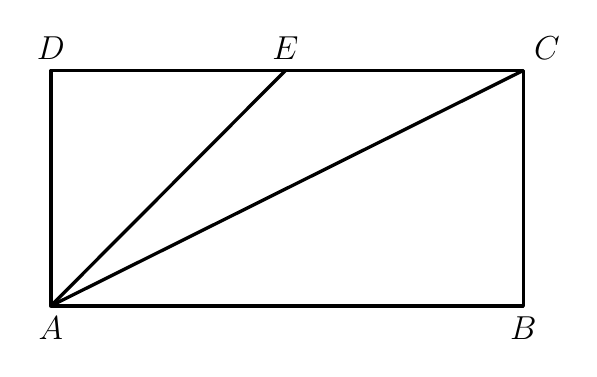
\begin{tikzpicture}[line width=1.2pt, line join=round]
  % Scale: 1 cm = 1/0.012685 px, so the 473 px width spans 6 cm
  \coordinate (D) at (0,0);
  \coordinate (C) at (6,0);
  \coordinate (B) at (6,-2.99);
  \coordinate (A) at (0,-2.99);
  \coordinate (E) at (2.98,0);   % midpoint of DC (approx.)

  % Rectangle ABCD
  \draw (A) -- (B) -- (C) -- (D) -- cycle;
  % Diagonal AC and segment AE
  \draw (A) -- (C);
  \draw (A) -- (E);

  % Vertex labels
  \node[above] at (D) {\fontsize{12}{14.4}\selectfont $D$};
  \node[above] at (E) {\fontsize{12}{14.4}\selectfont $E$};
  \node[above right] at (C) {\fontsize{12}{14.4}\selectfont $C$};
  \node[below] at (A) {\fontsize{12}{14.4}\selectfont $A$};
  \node[below] at (B) {\fontsize{12}{14.4}\selectfont $B$};
\end{tikzpicture}
\end{document}